%%%%%%%%%%%%%%%%%%%%%%%%%%%%%%%%%%%%%%%%%%%
\chapter{Elementos de Euclides}
\section{Definições}


\begin{defi}
Um ponto é o que não tem partes.
\end{defi}
\begin{enumerate}
 \item Um ponto é o que não tem partes.\\
 \begin{tikzpicture}
 \draw (0,0) node[circle, inner sep=2pt, fill=black, label={above:{$x$}}] (x) {}
 \end{tikzpicture}
 
 \item Uma línha tem comprimento mas não tem largura.\\
 \begin{tikzpicture}
 \draw (0,0) -- (1,0)
 \end{tikzpicture}
 \\
 \item Os extremos de uma línha são pontos.\\
 
 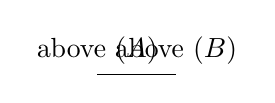
\begin{tikzpicture}
 \coordinate [label=above ($A$)] (A) at (0,0);
 \coordinate [label=above ($B$)] (B) at (1,0);
 
 \draw (A) -- (B);
 \end{tikzpicture}
 \item Uma superfície é aquela que só tem comprimento e largura.
 \item Os extremos de uma superfície são linhas.
 \item Superfície plana é aquela, sobre a qual assenta toda uma tinha reta entre dois pontos quaisquer, que estiverem na mesma superfície.
 \item Ângulo plano é a inclinação recíproca de duas linhas, qu se tocam em uma superfície plana, sem estarem em direitura uma com outra (sem estarem sobre uma mesma linha).
 \item Ângulo plano retilíneo é a inclinação recíproca de duas linhas retas, que se encontram, e não estão em direitura uma com outra.
 \item Um ângulo é a inclinação mutua de duas linhas que se encontram em um plano e não são colineares.
 \item Quando as línhas que compreendem o 

\end{enumerate}